%auto-ignore
\providecommand{\MainFolder}{..}
\documentclass[\MainFolder/Text.tex]{subfiles}


\begin{document}

\section{Chern-Simons Maurer-Cartan element} \label{Section:Proof2} 
%Proof of Proposition~\ref{Proposition:MCSphere} - 

We first recall ribbon graphs and their labelings based on~\cite{Cieliebak2015}. 

\begin{Definition}[Ribbon graph]\label{Def:Ribbon}
A \emph{graph} $\Gamma$ is a quadruple $(V,H,\mathcal{V},\mathcal{E})$, where~$V$ is a finite set of vertices, $H$ a finite set of half-edges, $\mathcal{V}: H \rightarrow V$ the ``vertex map'' and $\mathcal{E}: H \rightarrow H$ with $\mathcal{E} \circ \mathcal{E} = \Id$ and without fixed points the ``edge map''. The preimage $\mathcal{E}^{-1}(h_1) = \{h_1, h_2\}$ for some $h_1$, $h_2\in H$ is called an \emph{edge}; the set of edges is denoted by $E$. We assume that the graphs are \emph{connected}, i.e., that for any $\Vert_1$, $\Vert_2 \in V$ there exists a path in $E$ connecting $\Vert_1$ to $\Vert_2$.

A \emph{ribbon graph} is a graph $\Gamma$ together with a free transitive action $\Z_{d(\Vert)}\ \rotatebox[origin=c]{-90}{$\circlearrowright$}\  \mathcal{V}^{-1}(\Vert)$ for every $\Vert\in V$, where $$d(\Vert) \coloneqq \Abs{\mathcal{V}^{-1}(\Vert)} $$
is the \emph{valency of $\Vert$}. We denote by $\Succ: H \rightarrow H$ the bijection induced by $1\in \Z_{d(\Vert)}$ for every $\Vert\in V$.


For a ribbon graph $\Gamma$, consider the set of sequences $(h_n)_{n\in \Z} \subset H$ such that the following conditions holds:
$$ \forall n\in \Z: \quad  h_{n+1}= \begin{cases} 
\mathcal{E}(h_n) & n\text{ even,}\\                                
\Succ(h_n) & n\text{ odd.}
\end{cases}$$
Two such sequences $(h_n)_{n\in \Z}$ and $(h'_n)_{n\in \Z}$ are equivalent if and only if there exist $n_0$, $n'_0 \in \Z$ both even or both odd such that $h_{n_0} = h'_{n_0'}$. An equivalence class $[(h_n)_{n\in \Z}]$ is called a \emph{boundary (or a boundary component) of $\Gamma$.} The set of boundaries of $\Gamma$ is denoted by $\Bdd \Gamma$.

An \emph{IE ribbon graph} is a ribbon graph $\Gamma$ together with the decomposition $V = V_{\mathrm{int}} \sqcup V_{\mathrm{ext}}$ into \emph{internal} and \emph{external vertices} $V_{\mathrm{int}}$ and $V_{\mathrm{ext}}$, respectively, such that $d(\Vert) = 1$ for all $\Vert\in V_{\mathrm{ext}}$. This decomposition induces the decomposition $E = E_{\mathrm{int}} \sqcup E_{\mathrm{ext}}$, where an edge $\Edge$ is internal if it connects two internal vertices and is external otherwise. We allow only graphs with \emph{at least one internal vertex}. We often identify an external vertex with its unique adjacent half-edge or the unique adjacent external edge; we call either of these an \emph{external leg}. For any $\Boundary \in \Bdd \Gamma$, we define the \emph{valency of $\Boundary$} by
$$ s(\Boundary) \coloneqq \Abs{\mathcal{V}(\Boundary) \cap V_{\mathrm{ext}}}, $$
where $\mathcal{V}(\Boundary) = \{\mathcal{V}(h_n) \mid n\in \Z\}$. We also have the free transitive $\Z_{s(\Boundary)}$-action on $\mathcal{V}(\Boundary)\cap V_{\mathrm{ext}}$ mapping $\Vert\in \mathcal{V}(\Boundary) \cap V_{\mathrm{ext}}$ to the next external vertex in the sequence $(\mathcal{V}(h_n))_{n\in\Z}$. We will denote this action by $\mathcal{N}$ again.

We say that an IE ribbon graph $\Gamma$ is \emph{reduced} if $s(\Boundary) \ge 1$ for all $\Boundary\in \Bdd \Gamma$.

The following letters will be used to denote the numerical invariants of a graph:
$$\begin{aligned}
k &\;\,\dots && \text{the number of internal vertices}, \\
s &\;\,\dots && \makebox[\widthof{the number of}]{---\ditto---} \text{ external vertices.}\\
l &\;\,\dots && \makebox[\widthof{the number of}]{---\ditto---}\text{ boundary components,} \\
e &\;\,\dots && \makebox[\widthof{the number of}]{---\ditto---} \text{ internal edges.}
\end{aligned}$$
Moreover, we define the \emph{genus $g\in \N_0$} so that the following \emph{Euler formula} holds:
\begin{equation} \label{Eq:EulerFormula}
 k - e + l = 2 - 2g.
\end{equation}\par
We denote by $\RG_{klg}$ the set of isomorphism classes of connected IE ribbon graphs with fixed $k$, $l$, $g$. We let $\RRG_{klg} \subset \RG_{klg}$ be the subset of reduced graphs. For $m\in \N_0$, we denote by $\RG_{klg}^{(m)} \subset \RG_{klg}$ the set of isomorphism classes of connected IE ribbon graphs with all internal vertices \emph{m-valent}, i.e., with 
$$ d(\Vert) = m\quad\text{for all }\Vert\in V_{\mathrm{int}}. $$
The notation $\Gamma \in \RG_{klg}$ means that $\Gamma$ is a representative of an equivalence class $[\Gamma]\in \RG_{klg}$.
\end{Definition}

\begin{Remark}[On ribbon graphs]\phantomsection
\begin{RemarkList}
\item An $m$-valent ribbon graph with $m\ge 2$ has a unique decomposition $V = V_{\mathrm{int}}\sqcup V_{\mathrm{ext}}$, and hence we can omit writing IE.
\item In this text, we will use only reduced ribbon graphs. Non-reduced ribbon graphs may play a role in the extension of the theory of $\dIBL^\PMC(\CycC(\Harm))$ to non-reduced cyclic cochains  or in the weak $\IBLInfty$-theory (see Remarks \ref{Rem:BVForm} and~\ref{Rem:NWG}).\qedhere
\end{RemarkList}
\end{Remark}

\begin{Def}[Labeling] \label{Def:Labeling}
A \emph{labeling} of an IE ribbon graph $\Gamma$ is the triple $L = (L_1,L_2,L_3)$, where $L_i$ have the following meanings: 
\begin{itemize}
 \item The symbol $L_1$ represents an ordering of internal vertices ($\eqqcolon L_1^v$), and of boundary components ($\eqqcolon L_1^b$). Given $L_1$, we write $V_{\mathrm{ext}} = \{\Vert_1, \dotsc, \Vert_k\}$, $\Bdd \Gamma = \{\Boundary_1, \dotsc, \Boundary_l\}$ and denote
$$ d_i \coloneqq d(\Vert_i)\quad\text{and}\quad s_j\coloneqq s(\Boundary_j). $$
 \item The symbol $L_2$ represents an ordering and orientation of internal edges. Given $L_2$, we write $E_{\mathrm{int}} = \{\Edge_1, \dotsc, \Edge_e\}$ and $\Edge_i =\{h_{i,1}, h_{i,2}\}$ for $h_{i,1}$, $h_{i,2}\in H$.
 \item The symbol $L_3$ represents an ordering of half-edges at every internal vertex ($\eqqcolon L_3^v$) and of external vertices at every boundary component ($\eqqcolon L_3^b$), both compatible with the \emph{ribbon structure} ($\coloneqq$\,the $\Z_m$-actions). Given $L_3$, we write $\mathcal{V}^{-1}(\Vert) = \{h_{\Vert,1}, \dotsc,h_{\Vert,d(\Vert)} \}$ and $\mathcal{V}(\Boundary) \cap V_{\mathrm{ext}}= \{\Vert_{\Boundary,1},\dotsc,\Vert_{\Boundary,s(\Boundary)}\}$ with $\Succ(h_{\Vert,i}) = h_{\Vert,i+1}$ and $\Succ(\Vert_{\Boundary,j}) = \Vert_{\Boundary,j+1}$ for all $i$, $j$, respectively. 
\end{itemize}
We sometimes call $L_i$ \emph{partial labelings} and $L$ a \emph{full labeling}. A ribbon graph $\Gamma$ together with a labeling $L$ is called a \emph{labeled ribbon graph}.
\end{Def}

Given a ribbon graph $\Gamma$, one can construct an oriented surface with boundary~$\Sigma_\Gamma$ --- the thickening of $\Gamma$ --- in the obvious way and a closed oriented surface~$\hat{\Sigma}_\Gamma$ by gluing oriented disks to the oriented boundaries of $\Sigma_\Gamma$. If partial labelings~$L_1$ and~$L_2$ are given, we obtain the following chain complex with oriented chain groups (vector spaces over $\R$):
\begin{equation} \label{Eq:OrientationComplex}
\begin{tikzcd}
C_2\coloneqq \langle \Boundary_1,\dotsc,\Boundary_l \rangle \arrow{r}{\Bdd_2} & C_1\coloneqq \langle \Edge_1,\dotsc, \Edge_e \rangle \arrow{r}{\Bdd_1} &  C_0\coloneqq \langle \Vert_k,\dotsc, \Vert_1 \rangle.
\end{tikzcd}
\end{equation}
Here $\Boundary_i$ stands for the oriented disc glued to the $i$-th boundary component of~$\Sigma_\Gamma$ and now being mapped into $\hat{\Sigma}_\Gamma$, $\Edge_i$ stands for the $1$-simplex in $\hat{\Sigma}_\Gamma$ corresponding to the $i$-th internal edge, $\Vert_i$ stands for the $0$-simplex in $\hat{\Sigma}_\Gamma$ corresponding to the $i$-th internal vertex, and the boundary map $\Bdd$ is the ``geometric'' boundary operator. The homology of this chain complex is isomorphic to the singular homology $\H(\hat{\Sigma})\coloneqq\H(\hat{\Sigma}_\Gamma;\R)$.

The orientation of $C_i$ ($\coloneqq$\,the order of generators in \eqref{Eq:OrientationComplex}) induces naturally an orientation of $\H(\hat{\Sigma}_\Gamma)$. The construction from \cite[Appendix A]{Cieliebak2015} is as follows. We pick complements $H_i$ of $\Im(\Bdd_{i+1})$ in $\Ker(\Bdd_{i})$ and complements $V_i$ of $\Ker(\Bdd_i)$ in $C_i$ and write 
$$\begin{tikzcd}
C_2 = V_2 \oplus H_2 \arrow{r}{\Bdd_2} & C_1 = V_1 \oplus H_1 \oplus \Im(\Bdd_2) \arrow{r}{\Bdd_1} & C_0 = \Im(\Bdd_1) \oplus H_0.
\end{tikzcd}$$
We orient $V_i$ arbitrarily and transfer the orientation to $\Im(\Bdd_{i})$ via  $\Bdd_{i} : V_i \overset{\simeq}{\rightarrow} \Im(\Bdd_{i})$. Then, assuming the direct sum orientation, orienting $H_i$ is equivalent to orienting $C_i$, and we obtain the orientation of $\H_i(\hat{\Sigma}_\Gamma)$ via the canonical projection $\pi: H_i \overset{\simeq}{\rightarrow} \H_i(\hat{\Sigma}_\Gamma) = \Ker(\Bdd_i)/\Im(\Bdd_{i+1})$. This construction does not depend on the choices of complements and orientations of $V_i$.

\begin{Definition}[Compatibility of $L_1$ and $L_2$]\label{Def:CompatLabeling}
Given a ribbon graph $\Gamma$ with partial labelings $L_1$ and $L_2$, we say that \emph{$L_2$ is compatible with $L_1$} if the orientation on $\H(\widehat{\Sigma}_\Gamma)$ induced by \eqref{Eq:OrientationComplex} agrees with the canonical orientation $$\H(\widehat{\Sigma}_\Gamma) =  \langle \Vert_1 + \dotsb + \Vert_k \rangle  \oplus \H_1(\widehat{\Sigma}_\Gamma) \oplus \langle \Boundary_1 + \dotsb + \Boundary_l\rangle, $$
where $\H_1(\widehat{\Sigma}_\Gamma)$ is oriented using the canonical symplectic intersection form.
\end{Definition}

Given a labeled IE ribbon graph $\Gamma$, the set of half-edges adjacent to internal vertices $\mathcal{V}^{-1}(V_{\mathrm{int}})$ can be ordered in two ways corresponding to writing 
$$ 2e + (s_1+ \dotsb +s_l) = d_1+ \dotsb +d_k. $$
This leads to the following definition.
\begin{Definition}[Edge order and vertex order]\label{Def:EdgeVertex}
For a labeled IE ribbon graph~$\Gamma$, we define the following two orders on the set of half-edges $H$:
\begin{itemize}
\item \emph{Edge order:} The first $2e$ half-edges $h_{i,j}^{\mathrm{e}}$ are the ones from internal edges; they are ordered according to $L_2$. They are followed by blocks of $s_1$,~$\dotsc$, $s_l$ half-edges $h_{i,j}^{\Boundary}$ which come from the boundary components $i=1$,~$\dotsc$, $l$, respectively, and which are ordered according to $L_3^b$ inside the blocks. Schematically, we have
$$ (h_{1,1}^{\Edge} h_{1,2}^{\Edge})\dots(h_{e,1}^{\Edge} h_{e,2}^{\Edge})(h^{\Boundary}_{1,1}\dots h^{\Boundary}_{1,s_1})\dots(h^{\Boundary}_{l,1}\dots h^{\Boundary}_{l,s_l}). $$
\item \emph{Vertex order:} It consists of blocks of $d_1$,~$\dotsc$, $d_k$ half-edges $h_{i,j}^{\Vert}$ which come from internal vertices $1$,~$\dotsc$, $k$, and which are ordered according to $L_3^v$ inside the blocks. Schematically, we have
$$ (h_{1,1}^{\Vert}\dots h_{1,d_1}^{\Vert})\dots (h_{k,1}^{\Vert}\dots h_{k,d_k}^{\Vert}). $$
\end{itemize}
	
	We denote by $\sigma_L \in \Perm_{\Abs{H}}$ the \emph{permutation from the edge to the vertex order} which is constructed such that the $i$-th half-edge in the edge order is the same as the $\sigma_L(i)$-th half-edge in the vertex order.
\end{Definition}


From now on, we will consider only reduced trivalent ribbon graphs $\TRRG_{klg}$ with $k$, $l \ge 1$, $g\ge 0$. We will often use the equation
\begin{equation} \label{Eq:TrivalentFormula}
2e + s = 3k.
\end{equation}

\begin{Def}[Chern-Simons Maurer-Cartan element]
%\marginnote{Make reasoning why the integrals are well defined, i.e. why the product of $L^1$ Hodge propagators is again $L^1$?} 
\label{Def:PushforwardMCdeRham}
Let $M$ be an oriented closed Riemannian manifold, and let $\Prpg \in \DR^{n-1}(\Bl_\Diag(M\times M))$ be an admissible Hodge propagator from Definition~\ref{Def:GreenKernel}. The \emph{Chern-Simons Maurer-Cartan element $\PMC$}, or \emph{formal pushforward Maurer-Cartan element}, is the collection of 
$$ \PMC_{lg}\in \hat{\Ext}_l \CycC(\Harm(M))\quad\text{for all }l\ge 1, g\ge 0 $$
defined on generating words $\omega_i = \alpha_{i1} \dots \alpha_{is_i}\in \BCyc \Harm(M)$, where $\alpha_{ij} = \SuspU \eta_{ij}$ with $\eta_{ij}\in \Harm(M)$ for $s_i\ge 1$ and $i=1, \ldots, l$, 
%with homogenous $\alpha_{ij} = \Susp \eta_{ij} \in \Harm(M)[1]$
by the formula
\begin{equation}
\label{Eq:PushforwardMCdeRham}
\begin{aligned} 
& \PMC_{lg}(\Susp^{l} \omega_1 \otimes \dotsb \otimes \omega_l) \\ 
& \qquad \coloneqq \frac{1}{l!}\sum_{[\Gamma]\in \TRRG_{klg}} \frac{1}{\Abs{\Aut(\Gamma)}} (-1)^{s(k,l) + P(\omega)} \sum_{L_1,\,L_3^b} (-1)^{\sigma_L} I(\sigma_L),
\end{aligned}
\end{equation}
which we explain as follows:
\begin{itemize}
\item %The first sum is over all isomorphism classes of trivalent ribbon graphs $[\Gamma]$.
The second sum is over all partial labelings $L_1$ and $L_3^b$ of a representative~$\Gamma$ of~$[\Gamma]$. In every summand, we complete $L_1$ and $L_3^b$  to a full labeling $L = (L_1, L_2, L_3)$ by picking an arbitrary $L_3^v$ and an arbitrary $L_2$ compatible with $L_1$.

\item Suppose that $\Gamma$ and $L_1$ are \emph{admissible} with respect to the input $\omega_1$, $\dotsc$, $\omega_l$; this means that $\Gamma$ has $l$ boundary components and that the $i$-th boundary component has valency $s_i$ for every $i=1$, $\dotsc$, $l$. In this case, denoting $\sigma = \sigma_L$, we define
\begin{equation} \label{Eq:ISigma}
I(\sigma_L) \coloneqq \begin{multlined}[t]\int_{x_1,\dotsc,x_k} \Prpg(x_{\xi(\sigma_1)},x_{\xi(\sigma_2)}) \dotsm \Prpg(x_{\xi(\sigma_{2e-1})},x_{\xi(\sigma_{2e})}) \\ \eta_{11}(x_{\xi(\sigma_{2e+1})}) \dotsm \eta_{ls_{l}}(x_{\xi(\sigma_{2e+s})}),\end{multlined}
\end{equation}
where $\xi: \{1,\dotsc, 3k\} \rightarrow \{1,\dotsc,k\}$ is the function defined by 
$$ \xi(3j-2) = \xi(3j-1) = \xi(3j) \coloneqq j $$ for all $j=1, \dotsc, k$, $s = s_1 + \dotsb + s_l$, $\eta_{}(x_i)$ denotes the pullback of $\eta$ along the canonical projection $\pi_i: M^{\times k} \rightarrow M$ to the $i$-th component $M_i$, $\Prpg(x_i, x_j)$ denotes the pullback of $\Prpg$ along $\pi_{i} \times \pi_j : M^{\times k} \rightarrow M_i \times M_j$, and $\int_{x_1,\dotsc,x_k}$ denotes the integral of an $nk$-form over $k$ copies of $M$.

If $\Gamma$ and $L_1$ are not admissible, then we set $I(\sigma_L)\coloneqq 0$.
\item $s(k,l) \coloneqq k + kl(n-1) + \frac{1}{2} k(k-1) n \mod 2$.
\item $P(\omega) \coloneqq  \sum_{i=1}^l \sum_{j=1}^{s_i} (s - s_1 - \dotsb - s_{i-1} - j) \eta_{ij} \mod 2$.
\end{itemize}
\end{Def}
\noindent %The sum is finite using~\eqref{Eq:TrivalentFormula}. The summands are independent of a representant of $[\Gamma]$ and of the choice of $L_3^v$ and an $L_2$ compatible with $L_1$ and the symmetry properties hold. 
%Well-definedness is checked in Appendix~\ref{Section:Appendix} for the case when $\Prpg$ is decomposable and can be checked also in the de Rham case. 
In order to show that $\PMC_{lg}$ is well-defined and that the collection $(\PMC_{lg})$ satisfies Definition~\ref{Def:MaurerCartan} for $\dIBL(\CycC(\Harm(M)))$, there are several things to check:
\begin{PlainList}
 \item The integral $I(\sigma_L)$ converges.
 \item The sums are finite.
 \item The product $(-1)^{\sigma_L} I(\sigma_L)$ is independent of the choice of $L_3^v$ and $L_2$ compatible with $L_1$.
 \item The sum over labelings is independent of the chosen representative $\Gamma$ in an isomorphism class from $\TRRG_{klg}$.
  \item The map $\PMC_{lg}: \BCyc\Harm(M)[3-n]^{\otimes l} \rightarrow \R$ is graded symmetric on permutations of its inputs $\Susp\omega_i$.
 \item The map $\PMC_{lg}$ is graded symmetric on cyclic permutations of the components $\alpha_{ij}$ of each $\omega_{i}$.
 \item The degree condition 1) from Definition \ref{Def:MaurerCartan} holds with $d = n-3$.
 \item The filtration-degree condition 2) from Definition \ref{Def:MaurerCartan} holds with $\gamma = 2$.
 \item The Maurer-Cartan equation \eqref{Eq:MaurerCartanEquation} holds.
\end{PlainList}

Condition 9) will be proven in~\cite{Cieliebak2018} using the theory of iterated blow-ups.

Condition 1) follows from the property (P1) of a Hodge propagator~ $\Prpg$.
The idea is to associate one integration variable to each internal half-edge, obtaining the space $\{x_i^{(1)},x_i^{(2)},x_i^{(3)}\mid i=1, \dotsc, k\}$, and blowing-up pairs of variables connected by internal edges.
By (P1), the integrand of \eqref{Eq:ISigma} lifts to a smooth form on such a space.
The integral $\int_{x_1 \dotsc x_k}$ is then realized as an integral over the closure of a lift of the subspace $\{x_i^{(1)} = x_i^{(2)} = x_i^{(3)}\}$.
By compactness, the integral converges.
A detailed proof is under preparation in~\cite{Cieliebak2018}.

In this text, \underline{we will take 1) and 9) for granted.} 

\begin{Lemma} \label{Lem:MCCond}
Conditions 2) -- 8) hold.
\end{Lemma}
\begin{proof}

As for 2), the fixed input $\omega_1$, $\dotsc$, $\omega_l$ fixes the number $s$ of external vertices of $\Gamma$ by admissibility. Expressing $e$ from~\eqref{Eq:EulerFormula} and plugging it  in~\eqref{Eq:TrivalentFormula} gives
\begin{equation} \label{Eq:MCk}
k = s + 2 l + 4g - 4.
\end{equation}
We see that all parameters are fixed. Now, there is only finitely many elements with fixed $s$ in $\TRRG_{klg}$, and each of them has only finitely many labelings. Therefore, the sums are finite.

As for 3), we have to consider the orientation of the complex~\eqref{Eq:OrientationComplex}. Clearly, if two $L_2$'s are compatible with $L_1$, then they differ by an even number of the following operations: a~transposition of two internal edges or a change of the orientation of an internal edge. The former operation introduces no sign in $(-1)^{\sigma_L}$ but generates the sign $(-1)^{n-1}$ in $I(\sigma_L)$ from swapping the corresponding~$\Prpg$'s. The latter operation induces the sign $-1$ in $(-1)^{\sigma_L}$ and the sign $(-1)^n$ in $I(\sigma_L)$ from the symmetry $\Prpg(x,y) = (-1)^n \Prpg(y,x)$. Because the overall signs in $(-1)^{\sigma_L} I(\sigma_L)$ are the same, an even number of these operations preserves $(-1)^{\sigma_L} I(\sigma_L)$. This implies the independence of an $L_2$ compatible with~$L_1$. A~change in $L_3^v$ produces no sign in $(-1)^{\sigma_L}$ because every internal vertex is trivalent and a cyclic permutation of an odd number of elements is even. The integral $I(\sigma_L)$ remains unchanged because the change in $\sigma_L$ is compensated by the composition with $\xi$. Independence of the choice of $L_3^v$ follows.

As for 4), every isomorphism of ribbon graphs $\Gamma \rightarrow \Gamma'$ induces the bijection $L\mapsto L'$ of compatible labelings such that $\sigma_L = \sigma_{L'}$ ($L'$ is the ``pushforward'' labeling). The independence of the choice of a representative of $[\Gamma]$ follows.

As for 5), let $\mu\in \Perm_l$ be a permutation of the inputs $\Susp \omega_1$, $\dotsc$, $\Susp \omega_l$. The set of graphs which admit an admissible labeling is the same for both $\PMC_{lg}(\Susp^l \omega_1 \otimes \dotsb \otimes \omega_l)$ and $\PMC_{lg}(\Susp^l \omega_{\sigma_{1}^{-1}} \otimes \dotsb \otimes \omega_{\sigma_l^{-1}})$; we will pick one such $\Gamma$ and study the admissible labelings $L$ and $L'$, respectively. We write $\eta_i = \eta_{i1}\dots \eta_{i s_i}$ and $\Omega_i = \Susp \omega_i$ for all $i$, $j$, and denote by $I'(\sigma_{L'})$ the integral in the definition of $\PMC_{lg}(\Susp^l \omega_{\mu_1^{-1}} \otimes \dotsb \otimes \omega_{\mu_l^{-1}})$. Let $\tilde{\mu}\in \Perm_{3k}$ be the permutation which acts as the identity on $1$, $\dotsc$, $2e$ and as the block permutation determined by $\mu$ on $2e + 1$,~$\dotsc$, $2e+s$ divided into $l$ blocks of lengths $s_1$, $\dotsc$, $s_l$. For any $\sigma\in \Perm_{3k}$, we have
$$ \begin{aligned}
I'(\sigma) & = \begin{multlined}[t]\int_{x_1,\dotsc,x_k}\!\! \Prpg(x_{\xi(\sigma_1)},x_{\xi(\sigma_2)}) \dotsm \Prpg(x_{\xi(\sigma_{2e-1})},x_{\xi(\sigma_{2e})}) \\ \eta_{\mu_1^{-1} 1}(x_{\xi(\sigma_{2e+1})}) \dots \eta_{\mu_l^{-1} s_{\mu_l^{-1}}}(x_{\xi(\sigma_{2e+s})})\end{multlined} \\
 & = \begin{multlined}[t]\varepsilon(\mu,\eta) \int_{x_1,\dotsc,x_k} \!\! \Prpg(x_{\xi((\sigma\circ\tilde{\mu})_1)},x_{\xi((\sigma\circ\tilde{\mu})_2)}) \dotsm \Prpg(x_{\xi((\sigma\circ \tilde{\mu})_{2e-1})},x_{\xi((\sigma\circ\tilde{\mu})_{2e})}) \\ \eta_{11}(x_{\xi((\sigma\circ \tilde{\mu})_{2e+1})})\dots  \eta_{ls_l}(x_{\xi((\sigma\circ \tilde{\mu})_{2e+s})})\end{multlined} \\
 & = \varepsilon(\mu,\eta) I(\sigma \circ \tilde{\mu}).
\end{aligned} $$
The precomposition with $\tilde{\mu}$ corresponds to a bijection $(L_1,L_3^b)\mapsto (L_1', {L_3^{b}}')$ of partial labelings for $\PMC_{lg}(\Susp^l \omega_1 \dots \omega_l)$ and $\PMC_{lg}(\Susp^l \omega_{\mu_1^{-1}} \otimes \dotsb \otimes \omega_{\mu_l^{-1}})$, respectively. However, if $L_2$ is compatible with $L_1$, then in order to get an $L_2'$ compatible with $L_1'$, the labeling~$L_2$ has to be altered by as many operations of switching two internal edges or changing the orientation of an internal edge as there are transpositions in $\mu$. We explained in the proof of 3) that this produces the sign $(-1)^{(n-1)\mu}$ in $(-1)^{\sigma_{L'}}I(\sigma_{L'})$. Therefore, after the choice of compatible $L_2$ and~$L_2'$, we have
$$ (-1)^{\sigma_{L'}}I'(\sigma_{L'}) = (-1)^{(n-1)\mu} (-1)^{\tilde{\mu}} \varepsilon(\mu, \eta) (-1)^{\sigma_L} I(\sigma_L). $$ 
If we view $\eta$ as $\eta_{11} \dots \eta_{l s_l}$, we can understand $(-1)^{P(\omega)}$ as the Koszul sign $\varepsilon(\SuspU, \eta)$. Similarly, we write $(-1)^{P(\mu(\omega))}=\varepsilon(\SuspU,\mu(\eta))$, where we first view $\eta$ as $\eta_1 \otimes \dotsb \otimes \eta_l$ to apply $\mu$ and then as the list of components $\eta_{ij}$ to compute the Koszul sign (this is a little ambiguity in our notation). If we denote by $\widebar{\mu}$ the permutation of $1$, $\dotsc$, $s$ permuting the $l$ blocks of lengths $s_1$, $\dotsc$, $s_l$ according to $\mu$, then $\widebar{\mu}$ has the same sign as $\tilde{\mu}$, and the decomposition of $\varepsilon(\SuspU,\mu(\eta))$ into the moves
$$ \begin{aligned}
\SuspU_{1} \dots \SuspU_{s} \eta_{\mu_1^{-1}1} \dots \eta_{\mu_l^{-1} s_{\mu_l^{-1}}} &\xrightarrow{(1)} \SuspU_{\widebar{\mu}_{1}} \dots \SuspU_{\widebar{\mu}_{s}} \eta_{11} \dots \eta_{l s_l} \xrightarrow{(2)} \SuspU_{\widebar{\mu}_1} \eta_{11} \dots \SuspU_{\widebar{\mu}_s} \eta_{l s_l} \\ &\xrightarrow{(3)} \SuspU_{1} \eta_{\mu_1^{-1}1} \dots \SuspU_{s} \eta_{\mu_l^{-1} s_l} \end{aligned} $$
shows that
$$ (-1)^{P(\mu(\omega))} = \underbrace{(-1)^{\tilde{\mu}}\varepsilon(\mu,\eta)}_{(1)} \underbrace{(-1)^{P(\omega)}}_{(2)}\underbrace{\varepsilon(\mu,\omega)}_{(3)}. $$
Using this, we write
$$ (-1)^{P(\mu(\omega))} (-1)^{\sigma_{L'}} I'(\sigma_{L'}) = \varepsilon(\mu,\omega) (-1)^{(n-1)\mu} (-1)^{P(\omega)}(-1)^{\sigma_L} I(\sigma_L), $$
and compute
$$ \begin{aligned}
& \PMC_{lg}(\Omega_{\mu_1^{-1}} \otimes \dotsb \otimes \Omega_{\mu_l^{-1}}) \\ & \qquad =\varepsilon(\mu(\Susp), \mu(\omega)) \PMC_{lg}(\Susp^l \omega_{\mu_1^{-1}} \otimes \dotsb \otimes \omega_{\mu_l^{-1}}) \\ 
& \qquad= \varepsilon(\mu(\Susp), \mu(\omega)) (-1)^{\Abs{s}\mu} \varepsilon(\mu,\omega) \PMC_{lg}(\Susp^l \omega_{1} \otimes \dotsb \otimes \omega_{l}) \\
& \qquad= \underbrace{\varepsilon(\mu(\Susp), \mu(\omega))}_{(1)} \underbrace{(-1)^{\Abs{s}\mu} \varepsilon(\mu,\omega)}_{(2)} \underbrace{\varepsilon(\Susp,\omega)}_{(3)} \PMC_{lg}(\Susp\omega_{1} \otimes \dotsb \otimes \Susp \omega_{l}) \\
& \qquad= \varepsilon(\mu,\Omega) \PMC_{lg}(\Omega_{1} \otimes \dotsb \otimes \Omega_{l}).
\end{aligned} $$
We used $\Abs{s} = n-1\text{ mod }2$, and the last equality follows from the decomposition of $\varepsilon(\mu,\Omega)$ into the moves
$$  \begin{multlined} \Susp_1 \omega_1 \dots \Susp_l \omega_l \xrightarrow{(3)} \Susp_1 \dots \Susp_l \omega_1 \dots \omega_l \xrightarrow{(2)} \Susp_{\mu_1^{-1}}\dots \Susp_{\mu_l^{-1}} \omega_{\mu_1^{-1}} \dots \omega_{\mu_l^{-1}} \\ \xrightarrow{(1)} \Susp_{\mu_1^{-1}} \omega_{\mu_1^{-1}} \dots \Susp_{\mu_l^{-1}} \omega_{\mu_l^{-1}}. \end{multlined}$$
This proves the symmetry of $\PMC_{lg}$.


As for 6), fix an $i=1$, $\dotsc$, $l$ and let $\mu\in \Perm_{s_i}$ be a cyclic permutation permuting the components of $\omega_i = \alpha_{i1}\dots \alpha_{is_i}$. Similarly to the previous case, we denote by~$\tilde{\mu}$ the corresponding permutation of $1$, $\dotsc$, $3k$ and get a bijection $(L_1,L_3^b) \mapsto (L_1'=L_1,{L_3^b}')$ of admissible labelings of a given graph $\Gamma$ for $\PMC_{lg}(\Susp^l \omega_1 \otimes \dotsb \otimes \alpha_{i1}\dots \alpha_{is_i} \otimes \dotsb \otimes \omega_l)$ and $\PMC_{lg}(\Susp^l \omega_1 \otimes \dotsb \otimes \alpha_{i\mu_1^{-1}} \dots \alpha_{i\mu_{s_i}^{-1}}\otimes \dotsb \otimes \omega_l)$, respectively. This time, there is no change in $L_1$, and thus we can take $L_2'=L_2$, producing no sign. Therefore, we have
$$ (-1)^{\sigma_{L'}}I'(\sigma_{L'}) = (-1)^{\tilde{\mu}}\varepsilon(\mu,\eta_i)(-1)^{\sigma_{L}}I(\sigma_{L}), $$
where $\varepsilon(\mu,\eta_i)$ comes from permuting the forms in $I'(\sigma_{L'})$. Further, we deduce
$$ (-1)^{P(\mu(\omega))} = (-1)^{\tilde{\mu}} \varepsilon(\mu,\eta_i) (-1)^{P(\omega)} \varepsilon(\mu,\omega_i), $$
and hence
$$ \begin{aligned}
&\PMC_{lg}(\Susp^l \omega_1 \otimes \dotsb \otimes \alpha_{i\mu_1^{-1}} \dots \alpha_{i\mu_{s_i}^{-1}}\otimes \dotsb \otimes \omega_l) \\
&\qquad = \varepsilon(\mu,\omega_i) \PMC_{lg}(\Susp^l \omega_1 \otimes \dotsb \otimes \alpha_{i1}\dots \alpha_{is_i}\otimes\dotsb\otimes \omega_l ). \end{aligned}$$
This shows the symmetry of $\PMC_{lg}$ on cyclic permutations of the components of~$\omega_i$.

As for 7), suppose that $\PMC_{lg}(\Susp^l \omega_1 \otimes \dotsb \otimes \omega_l) \neq 0$, and let $D$ denote the total form-degree of the input $\eta_{11}$, $\dotsc$, $\eta_{l s_l}\in \Harm(M)$; i.e., we define
\begin{equation*}
 D \coloneqq \deg(\eta_{11}) + \dotsb + \deg(\eta_{1s_1}) + \dotsb + \deg(\eta_{l 1}) + \dotsb + \deg(\eta_{l s_l}).
\end{equation*}
Clearly, we must have
\begin{equation}  \label{Eq:TotDeg}
nk = (n-1) e  + D, 
\end{equation}
where the left-hand side is the dimension of $M^{\times k}$ and the right-hand side the form-degree of the integrand of $I(\sigma_L)$. If we plug in $e$ from~\eqref{Eq:EulerFormula} and $k$ from~\eqref{Eq:MCk}, we get
$$ \begin{aligned} D &= nk - (n-1) e \\ 
   &= nk - (n-1)(k+l+2g-2) \\
   & = k - (n-1)(l+2g-2) \\
   & = s + 2l +4g - 4 - (n-1)(l+2g-2) \\
   & = s - (n-3)(l+2g-2). \end{aligned}$$
It follows that
$$ \Abs{\PMC_{lg}} = \Abs{\Susp^l} + \Abs{\omega_1} +  \dotsb + \Abs{\omega_l} =  l(n-3) + D - s = - 2(n-3)(g-1). $$
This is exactly the degree from Definition~\ref{Def:MaurerCartan}. 

As for 8), if $\PMC_{lg}(\Susp^l \omega_1 \otimes \dotsb\otimes \omega_l)\neq 0$, then
$$ s = k - 2l -4g -4 \ge 1 + 2(2-2g-l) = 1 + 2 \chi_{0lg}, $$
and hence $\PMC_{lg}\in \Filtr^{1+2\chi_{0lg}}\hat{\Ext}_l \CycC$ for the filtration induced from the dual of the filtration of $\BCyc \Harm$ by weights. Therefore, we get 
$$ \|\PMC_{lg}\| \ge 1 + 2\chi_{0lg} > 2\chi_{0lg} \quad\text{for all }l\ge 1, g\ge 0. $$
This finishes the proof.
\end{proof}

\Modify[inline,caption={Superfluous signs}]{Add here a remark that we do not have to sum over $L_1^v$!.}
%In~\cite{Cieliebak2018}, however, they might use a different convention for~$s(k,l)$. Our signs come naturally from the formal analogy $\DR(M) \simeq V$, where $V$ is a finite-dimensional vector space with a non-degenerate pairing, under which the formal pushforward Maurer-Cartan element $\PMC$ induced from $\DR(M)$ becomes a genuine pushforward Maurer-Cartan element induced from $V$, which fits in the formalism of~\cite{Cieliebak2015}. See Appendix~\ref{Section:Appendix} for more details.

\begin{Definition}[Vertices of types A, B, C and some special graphs]\label{Def:Graphs}
Let $\Gamma \in \TRG_{klg}$ be a trivalent ribbon graph and $\Vert$ its internal vertex. We say that~$\Vert$ is of \emph{type $A$, $B$ or~$C$} if it is connected to precisely $1$, $2$ or~$3$ internal vertices, respectively (see Figure~\ref{Fig:Vertices}). The graph $\Gamma$ is called (see Figures~\ref{Fig:Types} and~\ref{Fig:YOk}):
\begin{itemize}
\item a \emph{tree} if $[\Gamma] \in \RG_{k10}$ for some $k\ge 1$;
\item \emph{circular} if $[\Gamma]\in \RG_{k20}$ for some $k\ge 1$;
\item the \emph{$Y$-graph} is the unique tree with $k=1$;
\item an \emph{$O_k$-graph} if $\Gamma$ is circular with $k$ internal vertices and no $A$-vertex.
\end{itemize}
We denote the $Y$-graph simply by $Y$.
\end{Definition}

{ \begingroup
\begin{figure}[t]
\centering
\begin{subfigure}{0.4\textwidth}
\centering
%auto-ignore
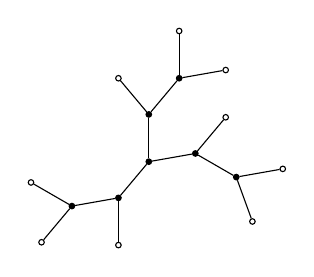
\begin{tikzpicture}

\def\rad{1cm}
\def\angdist{140}
\def\posa{90}
\def\extlen{0.6cm}

\tikzset{point/.style = {draw, circle, fill=black, minimum size=2pt,inner sep=0pt}}


\coordinate[point] (C1) at (0,0) {};
\path (C1) node[point] (C11)  at +(\posa:\extlen) {};
\path (C1) node[point] (C12)  at +(\posa+\angdist:\extlen) {};
\path (C1) node[point] (C13)  at +(\posa+2*\angdist:\extlen) {};
\draw (C1) -- (C11);
\draw (C1) -- (C12);
\draw (C1) -- (C13);

\path (C11) node[point] (C111)  at +(-180+\posa+\angdist:\extlen) {};
\path (C11) node[point,style={fill=white}] (C112)  at +(-180+\posa-\angdist:\extlen) {};
\draw (C11) -- (C111);
\draw (C11) -- (C112);

\path (C12) node[point] (C121)  at +(-180+\posa+\angdist + \angdist:\extlen) {};
\path (C12) node[point,style={fill=white}] (C122)  at +(-180+\posa+\angdist - \angdist:\extlen) {};
\draw (C12) -- (C121);
\draw (C12) -- (C122);

\path (C13) node[point] (C131)  at +(-180+\posa+2*\angdist + \angdist:\extlen) {};
\path (C13) node[point,style={fill=white}] (C132)  at +(-180+\posa+2*\angdist - \angdist:\extlen) {};
\draw (C13) -- (C131);
\draw (C13) -- (C132);


\path (C121) node[point,style={fill=white}] (C1211)  at +(-180-180+\posa+\angdist + \angdist+\angdist:\extlen) {};
\path (C121) node[point,style={fill=white}] (C1212)  at +(-180-180+\posa+\angdist + \angdist-\angdist:\extlen) {};
\draw (C121) -- (C1211);
\draw (C121) -- (C1212);

\path (C111) node[point,style={fill=white}] (C1112)  at +(-180-180+\posa+\angdist+\angdist:\extlen) {};
\path (C111) node[point,style={fill=white}] (C1111)  at +(-180-180+\posa+\angdist-\angdist:\extlen) {};
\draw (C111) -- (C1111);
\draw (C111) -- (C1112);

\path (C131) node[point,style={fill=white}] (C1312)  at +(-180-180+\posa+2*\angdist + \angdist+\angdist:\extlen) {};
\path (C131) node[point,style={fill=white}] (C1311)  at +(-180-180+\posa+2*\angdist + \angdist-\angdist:\extlen) {};
\draw (C131) -- (C1311);
\draw (C131) -- (C1312);

\end{tikzpicture}
\end{subfigure}
\begin{subfigure}{0.4\textwidth}
\centering
%auto-ignore
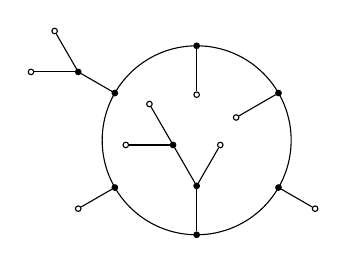
\begin{tikzpicture}

\def\rad{1.2cm}
\def\angdist{60}
\def\posa{90}
\def\extlen{0.6cm}

\tikzset{point/.style = {draw, circle, fill=black, minimum size=2pt,inner sep=0pt}}


\coordinate (C1) at (0,0) {};

\path (C1) node[point] (C11)  at +(\posa:\rad) {};
\path (C1) node[point] (C12)  at +(\posa+\angdist:\rad) {};
\path (C1) node[point] (C13)  at +(\posa+2*\angdist:\rad) {};
\path (C1) node[point] (C14)  at +(\posa+3*\angdist:\rad) {};
\path (C1) node[point] (C15)  at +(\posa+4*\angdist:\rad) {};
\path (C1) node[point] (C16)  at +(\posa+5*\angdist:\rad) {};


\draw (C1) circle (\rad);

% C1
\path (C1) to coordinate[pos=1-\extlen/\rad,point,style={fill=white}] (C111) (C11);
\draw (C11) -- (C111);


% C2
\path (C1) to coordinate[pos=1+\extlen/\rad,point] (C121) (C12);
\path (C121) node[point,style={fill=white}] (C1211)  at +(\posa+\angdist+30:\extlen) {};
\path (C121) node[point,style={fill=white}] (C1212)  at +(\posa+\angdist-30:\extlen) {};

\draw (C12) -- (C121);
\draw (C121) -- (C1211);
\draw (C121) -- (C1212);

% C3
\path (C1) to coordinate[pos=1+\extlen/\rad,point,style={fill=white}] (C131) (C13);
\draw (C13) -- (C131);


% C4
\path (C1) to coordinate[pos=1-\extlen/\rad,point] (C141) (C14);
\path (C141) node[point] (C142)  at +(120:\extlen) {};
\path (C141) node[point,style={fill=white}] (C143)  at +(60:\extlen) {};
\path (C142) node[point,style={fill=white}] (C1421)  at +(180:\extlen) {};
\path (C142) node[point,style={fill=white}] (C1422)  at +(120:\extlen) {};
\draw (C14) -- (C141);
\draw (C141) -- (C142);
\draw (C141) -- (C143);
\draw (C142) -- (C1421);
\draw (C142) -- (C1422);

% C5
\path (C1) to coordinate[pos=1+\extlen/\rad,point,style={fill=white}] (C151) (C15);
\draw (C15) -- (C151);

% C6
\path (C1) to coordinate[pos=1-\extlen/\rad,point,style={fill=white}] (C161) (C16);
\draw (C16) -- (C161);

\end{tikzpicture}
\end{subfigure}
\caption[A tree and a circular graph.]{A tree and a circular graph. Internal vertices are denoted with a full dot and external vertices with an empty dot.}\label{Fig:Types}
\end{figure}
\endgroup }
%
{ \begingroup
\begin{figure}[t]
\centering
\begin{subfigure}{0.4\textwidth}
\centering
%auto-ignore
\begin{tikzpicture}

\def\rad{1cm}
\def\angdist{120}
\def\posa{90}
\def\extlen{1.3cm}

\tikzset{point/.style = {draw, circle, fill=black, minimum size=2pt,inner sep=0pt}}


\coordinate[point] (C1) at (0,0) {};
\path (C1) node[point,style={fill=white}] (C11)  at +(\posa:\extlen) {};
\path (C1) node[point,style={fill=white}] (C12)  at +(\posa+\angdist:\extlen) {};
\path (C1) node[point,style={fill=white}] (C13)  at +(\posa+2*\angdist:\extlen) {};
\draw (C1) -- (C11);
\draw (C1) -- (C12);
\draw (C1) -- (C13);

\end{tikzpicture}
\end{subfigure}
\begin{subfigure}{0.4\textwidth}
\centering
%auto-ignore
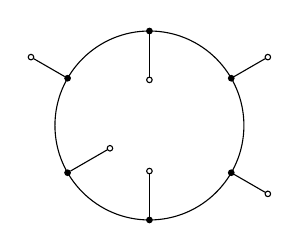
\begin{tikzpicture}

\def\rad{1.2cm}
\def\angdist{60}
\def\posa{90}
\def\extlen{0.6cm}

\tikzset{point/.style = {draw, circle, fill=black, minimum size=2pt,inner sep=0pt}}


\coordinate (C1) at (0,0) {};

\path (C1) node[point] (C11)  at +(\posa:\rad) {};
\path (C1) node[point] (C12)  at +(\posa+\angdist:\rad) {};
\path (C1) node[point] (C13)  at +(\posa+2*\angdist:\rad) {};
\path (C1) node[point] (C14)  at +(\posa+3*\angdist:\rad) {};
\path (C1) node[point] (C15)  at +(\posa+4*\angdist:\rad) {};
\path (C1) node[point] (C16)  at +(\posa+5*\angdist:\rad) {};


\draw (C1) circle (\rad);

% C1
\path (C1) to coordinate[pos=1-\extlen/\rad,point,style={fill=white}] (C111) (C11);
\draw (C11) -- (C111);


% C2
\path (C1) to coordinate[pos=1+\extlen/\rad,point,style={fill=white}] (C121) (C12);

\draw (C12) -- (C121);


% C3
\path (C1) to coordinate[pos=1-\extlen/\rad,point,style={fill=white}] (C131) (C13);
\draw (C13) -- (C131);


% C4
\path (C1) to coordinate[pos=1-\extlen/\rad,point,style={fill=white}] (C141) (C14);
\draw (C14) -- (C141);


% C5
\path (C1) to coordinate[pos=1+\extlen/\rad,point,style={fill=white}] (C151) (C15);
\draw (C15) -- (C151);

% C6
\path (C1) to coordinate[pos=1+\extlen/\rad,point,style={fill=white}] (C161) (C16);
\draw (C16) -- (C161);

\end{tikzpicture}
\end{subfigure}
\caption{The $Y$-graph and an $O_6$-graph.}\label{Fig:YOk}
\end{figure}
\endgroup }

\begin{Remark}[On $A$, $B$, $C$ vertices and special graphs]
We observe the following:
\begin{RemarkList}
\item A trivalent graph $\Gamma \neq Y$ has each internal vertex of type $A$, $B$ or $C$.
\item The term $\PMC_{10}$ is a sum over trees, and the term $\MC_{10}$ is the contribution of the $Y$-graph to $\PMC_{10}$ (see Proposition~\ref{Prop:FormalPushforwardProp} below). The term $\PMC_{20}$ is a sum over circular graphs.\qedhere
%The elements  of the Maurer-Cartan element are particularly important because they twist $\OPQ_{110}$, $\OPQ_{210}$, $\OPQ_{120}$ (c.f.~\eqref{Eq:TwisteddIBL}), and hence they are the only $\PMC_{lg}$ whose effect might be visible on the homology. See Section~\ref{Section:Proof3} for more details.\qedhere
\end{RemarkList}
\end{Remark}

Wee will also denote by $A$, $B$, $C$ the numbers of internal vertices of the corresponding type. Under the change of variables
\begin{equation} \label{Eq:ChangeOfVariables}
\begin{aligned}
  s &= 2 A + B, \\
  e &= B + \frac{1}{2} A + \frac{3}{2} C, \\
  k &= A + B + C,
\end{aligned}
\end{equation}
the trivalent formula~\eqref{Eq:TrivalentFormula} becomes trivial and the Euler formula~\eqref{Eq:EulerFormula} becomes
\begin{equation} \label{Eq:GenusFormulaa}
 C - A = 2l - 4 + 4g.
\end{equation}


\begin{Proposition}[Chern-Simons Maurer-Cartan element]\label{Prop:FormalPushforwardProp}
The collection $\PMC = (\PMC_{lg})$ from Definition~\ref{Def:PushforwardMCdeRham} is a Maurer-Cartan element for $\dIBL(\Harm(M))$ which is compatible with $\MC$. In particular, the $\AInfty$-algebra $\Harm(M)_\PMC$ is homologically unital and augmented.
\end{Proposition}
\begin{proof}
The fact that $\PMC$ is a Maurer-Cartan element follows from Lemma~\ref{Lem:MCCond} assuming 1) and 9) from \cite{Cieliebak2018}. \Correct[caption={DONE Redundant check of vanishing for $w\le 2$}]{Change it here because the definition of compatible changed!! In particular, the vanishing on words of length $1$ and $2$ follows from the filtration degree condition. Do not have to show it here.}

As for the compatibility with $\MC$,
%by plugging $l=1$, $g=0$ in \eqref{Eq:MCk}, we get $k = s-2$. Therefore, for all $\alpha_1$, $\alpha_2$, $\alpha_3\in\Harm(M)[1]$, we have $\PMC_{10}(\Susp \alpha_1) = \PMC_{10}(\Susp \alpha_1 \alpha_2) = 0$, and
the only graph contributing to $\PMC_{10}(\Susp \alpha_1 \alpha_2 \alpha_3)$  is the $Y$-graph with $k=1$. The group $\Aut(Y)$ consists of three rotations, and there is only one possible~$L_1$, no~$L_2$ and three~$L_3^b$. In Definition~\ref{Def:PushforwardMCdeRham}, we get $s(1,1) = n-2$, $(-1)^{\sigma_L} = 1$ because a cyclic permutation of an odd number of elements is even, and also $P(\alpha_1\alpha_2\alpha_3) =\eta_2$. Finally, we compute
\begin{align*}%\label{Eq:TheFirstTerm} 
 \PMC_{10}(\Susp \alpha_1 \alpha_2 \alpha_3) &= \frac{1}{3} (-1)^{n-2 + \eta_2}\sum_{L_3^b} \int_x \alpha_1(x_{\xi(\sigma_1)})\alpha_2(x_{\xi(\sigma_2)})\alpha_3(x_{\xi(\sigma_3)}) \\ 
 & = (-1)^{n-2 + \eta_2}\int_M \eta_1 \wedge \eta_2 \wedge \eta_3\\[\jot]
 & = \MC_{10}(\Susp \alpha_1 \alpha_2 \alpha_3).\qedhere
\end{align*}
\end{proof}
%
%Appendix~\ref{Section:Appendix}, which hold for a finite-dimensional vector space $V$, in the case of $\DR(M)$, replacing the product by the integral and a permutation of tensors by a change of variables. The formal analogy $V\sim \DR(M)$ is also used to get the signs $s(k,l)$ and $P(\omega)$, which is explained in details at the end of the Appendix. In~\cite{Cieliebak2018} will be argued, using iterated blow-ups, that the integrals $I(\sigma)$ converge, and that $\PMC=(\PMC_{lg})$ satisfies the Maurer-Cartan equation~\eqref{Eq:MaurerCartanEquation} with operations $\OPQ_{110}$, $\OPQ_{210}$ and $\OPQ_{120}$ from Definition~\ref{Def:CanonicaldIBL}. However, they might use a different convention for $s(k,l)$.
%%Our signs come from a formal analogy with the algebraic formalism in Appendix~\ref{Section:Appendix} which corresponds to a finite dimensional $\DR(M)$. In that case~\eqref{Eq:MaurerC1artanEquation} holds as  $(\MC_{10})$ is a Maurer-Cartan element and $(\PMC_{lg})$ its pushforward in the sense of~\cite{Cieliebak2015}. 


%In this section we will will work in the setting of Definition~\ref{Def:PushforwardMCdeRham}. To recall, we consider connected trivalent ribbon graphs $\Gamma$ with $k$ internal vertices, $l$ boundary components and genus $g$, the set of whose isomorphism classes is denoted by $RG_{klg}^{3}$; we label them using $L=(L_1,L_2,L_3)$ from Definition~\ref{Def:Labeling} and evaluate on an input $\omega_1$, $\dotsc$, $\omega_l \in \BCyc\Harm(M)$ with $\omega_i = \alpha_{i1}\dots \alpha_{is_i}$ for homogenous $\alpha_{ij}\in \Harm(M)[1]$  as the integral $I(\sigma_L)$. The value $\PMC_{lg}(\Susp^l \omega_1 \otimes \dotsb \otimes \omega_l)$  is then computed as a sum over $[\Gamma]\in RG_{klg}^3$ and all choices of an admissible labeling $L$
%
\begin{figure}[t]
\centering
%auto-ignore
\begin{tikzpicture}

\tikzset{point/.style = {draw, circle, fill=black, minimum size=2pt,inner sep=0pt}}

\def\dist{4}
\def\startangle{90}
\def\leglength{1.2}
\def\dashpart{0.5}

% The centers
\node[point,label={[xshift=-0.5cm,yshift=0.25cm]125:$A_{\alpha_1,\alpha_2}(y)$},label={-90:x}] (A) at (0,0) {};
\node[point,label={[xshift=-0.5cm,yshift=0.25cm]125:$B_\alpha(y_1,y_2)$},label={-90:x}] (B) at ($(A)+(\dist,0)$) {};
\node[point,label={[xshift=-0.5cm,yshift=0.25cm]125:$C(y_1,y_2,y_3)$},label={-90:x}] (C) at ($(A)+(2*\dist,0)$) {};

% Legs at the centers
\path (A) -- +(\startangle:\dashpart*\leglength) coordinate (A11) -- +(\startangle:\leglength) coordinate (A12);
\path (A) -- +(\startangle+120:\dashpart*\leglength) coordinate (A21) -- +(\startangle+120:\leglength) coordinate (A22);
\path (A) -- +(\startangle+240:\dashpart*\leglength) coordinate (A31) -- +(\startangle+240:\leglength) coordinate (A32);

\draw (A) -- (A12) node[point,style={fill=white},label={0:$\alpha_1$}] {};
\draw (A) -- (A22) node[point,style={fill=white},label={$\alpha_2$}] {};
\draw (A) -- (A31); \draw[dashed] (A31) -- (A32) node[at end,above]{y};



\path (B) -- +(\startangle:\dashpart*\leglength) coordinate (B11) -- +(\startangle:\leglength) coordinate (B12);
\path (B) -- +(\startangle+120:\dashpart*\leglength) coordinate (B21) -- +(\startangle+120:\leglength) coordinate (B22);
\path (B) -- +(\startangle+240:\dashpart*\leglength) coordinate (B31) -- +(\startangle+240:\leglength) coordinate (B32);

\draw (B) -- (B12) node[point,style={fill=white},label={0:$\alpha$}] {};
\draw (B) -- (B21); \draw[dashed] (B21) -- (B22) node[at end,above]{$y_1$};
\draw (B) -- (B31); \draw[dashed] (B31) -- (B32) node[at end,above]{$y_2$};


\path (C) -- +(\startangle:\dashpart*\leglength) coordinate (C11) -- +(\startangle:\leglength) coordinate (C12);
\path (C) -- +(\startangle+120:\dashpart*\leglength) coordinate (C21) -- +(\startangle+120:\leglength) coordinate (C22);
\path (C) -- +(\startangle+240:\dashpart*\leglength) coordinate (C31) -- +(\startangle+240:\leglength) coordinate (C32);

\draw (C) -- (C11); \draw[dashed] (C11) -- (C12) node[at end,above,right]{$y_1$};
\draw (C) -- (C21); \draw[dashed] (C21) -- (C22) node[at end,above]{$y_2$};
\draw (C) -- (C31); \draw[dashed] (C31) -- (C32) node[at end,above] {$y_3$};


%\path[draw] (C) -- +(\startangle:\leglength) node[at end,above,right]{int};
%\path[draw] (C) -- +(\startangle+120:\leglength) node[at end,above,yshift=2pt]{int};
%\path[draw] (C) -- +(\startangle+240:\leglength) node[at end,above,yshift=2pt]{int};

\end{tikzpicture}
\caption[Trivalent vertices of types $A$, $B$ and $C$.]{Trivalent vertices of types $A$, $B$ and $C$ with the corresponding forms $A_{\alpha_1,\alpha_2}$, $B_\alpha$ and $C$, respectively.}\label{Fig:Vertices}
\end{figure}
%
%
\begin{Definition}[Contributions of A, B, C vertices]\label{Def:Contributions}
Consider an internal vertex of type A, B or C as in Figure~\ref{Fig:Vertices}. We define the following smooth forms on $M$, $M^{\times 2}$ and $M^{\times 3}$, respectively:\footnote{The definitions can be made precise in local coordinates. Smoothness of $A_{\alpha_1, \alpha_2}$ is clear, smoothness of $B_\alpha$ follows from Lemma~\ref{Lem:Smoothing}, and smoothness of $C$ can be shown by a similar argument.}
$$\begin{aligned} 
 A_{\alpha_1, \alpha_2}(y)&\coloneqq \int_x \Prpg(y,x)\eta_1(x)\eta_2(x),\\ 
 B_\alpha(y_1,y_2) &\coloneqq \int_x \Prpg(y_1,x)\Prpg(x,y_2)\eta(x), \\
 C(y_1,y_2,y_3) &\coloneqq \int_x \Prpg(x,y_1)\Prpg(x,y_2)\Prpg(x,y_3).
\end{aligned}$$
\end{Definition}


\end{document}
